\documentclass[border=2pt]{standalone}
\usepackage{tikz}
\usetikzlibrary{backgrounds}
\begin{document}
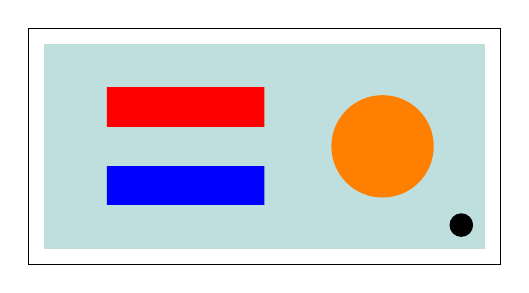
\begin{tikzpicture}
  \draw (0,0) rectangle (6,3);
  \begin{scope}
    \clip (1,.5) rectangle (3,2.5);
    \fill[red] (0,1.75) rectangle (6,2.25);
    \begin{scope}[on background layer]
      \fill[teal!25] (.2,.2) rectangle (5.8,2.8);
      \begin{scope}
        \clip (4.5,1.5) circle (.65cm);
        \fill[orange] (0,0) rectangle (6,3);
      \end{scope}
    \end{scope}
    \begin{scope}
      \fill[blue] (0,.75) rectangle (6,1.25);
    \end{scope}
  \end{scope}
  \fill[black] (5.5,.5) circle (.15cm);
\end{tikzpicture}
\end{document}
